%!TEX program = xelatex
\documentclass [a4paper]{article}
\author {SY1606407 王晓健}
\title {聚类与判别分析}
\usepackage{ctex}
\usepackage{amsmath}
\usepackage{amssymb}
\usepackage{booktabs}
\usepackage{geometry}
\usepackage{graphicx}
\usepackage{multirow}
\usepackage{tabu}
\geometry{left=2.5cm,right=2.5cm,top=2.5cm,bottom=2.5cm}
\begin{document}
\maketitle
\section{引言}
在过去30多年里,中国经济一直保持高速增长,所取得的成就令世人瞩目。从1978年到2013年,中国实现了年均9.8\%的国内生产总值(GDP)增长率,人均GDP实际增长17倍多。2016年,我国GDP远超日本,高居世界第二,城市化率也从1978年不到20\%上升到54.77\%。

但伴随着经济的迅速发展,区域发展不平衡的问题也日益显现。不同发展水平的城市在人口、经济、教育、房价等诸多方面往往有着较大的差异。根据多种统计数据对城市建立合理的分类模型可以很好地评估城市发展水平,衡量地区发展差异。对于引导政府的政策制定,促进资源的合理分配和区域之间的平衡发展,使得我国经济在『新常态』下实现平稳转型升级有着积极的意义。

本文提取了《中国统计年鉴2015》中2014年全国36个主要城市在年末总人口、区域生成总值、第三产业占比、社会商品零售总额、地方财政范围内收入、在岗职工平均工资、房地产开发投资金额、商品房销售价格、普通高校在校学生、城乡居民储蓄年末余额这10项指标上的统计数据,使用R语言建立了主成分聚类的方法对各个城市进行聚类分析,将主要城市分为5类,并利用线性判别分析的方法对聚类结果进行评估和分析。
\section{数据采集}
本文使用了《中国统计年鉴2015》中2014年全国包括北京、天津、石家庄、太原、呼和浩特、沈阳、大连、长春、哈尔滨、上海、南京、杭州、宁波、合肥、福州、厦门、南昌、济南、青岛、郑州、武汉、长沙、广州、深圳、南宁、海口、重庆、成都、贵阳、昆明、西安、兰州、西宁、银川、乌鲁木齐在内的36个主要城市在年末总人口、区域生成总值、第三产业占比、社会商品零售总额、地方财政范围内收入、在岗职工平均工资、房地产开发投资金额、商品房销售价格、普通高校在校学生、城乡居民储蓄年末余额这10项统计数据。各项指标的分布情况如表1所示
\begin{table}[h]
\centering
\caption{主各项指标的分布情况}
\small %此处写字体大小控制
\begin{tabular}{ccccccc}
\toprule
&指标&变化范围&均值 &中位数 &数据变差\\
\midrule

年末总人口    &      -0.234 & 0.518 & 0.130 & 0.468 & 0.353  \\
区域生产总值  &      -0.382 &  & 0.127 & -0.125 &    & 0.317 \\
第三产业占比   &     -0.165 & -0.420 & -0.729 & 0.482&      \\
社会商品零售总额   &  -0.387 &     &     &-0.102 &     &   \\
地方财政预算内收入  & -0.375 &     & 0.180 & 0.131 & -0.243 & 0.188 \\
在岗职工平均工资  &  -0.339 & -0.273 & 0.112 & -0.149 & -0.533 &        \\
房地产开发投资金额  & -0.341 & 0.274 &      & 0.165 &    & -0.860     \\
商品房销售价格  &    -0.268 & -0.433 & 0.149 & -0.355 & 0.714     \\
普通高等学校在校学生& -0.176& 0.455 & -0.605 & -0.566 &       &       \\
城乡居民储蓄年末余额&  -0.385&     &      &    &-0.104&   \\
\bottomrule
\end{tabular}
\end{table}
\section{主成分聚类分析}
由于所取数据中涉及的特征较多,也为了避免多个特征之间存在较强的相关关系使得距离度量失衡,聚类效果变差,本文选择使用主成分聚类的方法进行聚类分析。

主成分分析法由 K. Pearson 在1901年提出,是一种可以将多项相关指标化为少数几个不相关综合指标的降维方法。聚类分析则是数理统计中的一种多元分析方法, 它使用数学方法定量地确定样本的亲疏关系,从而对样本进行合理地划分。所谓主成分聚类分析就是将主成分分析与聚类分析相结合的一种综合评价方法,即先作主成分分析,再进行聚类分析。
    \subsection{主成分分析}
    	对于 p 元总体 $ x=(x_1,x_2,...,x_p)$ 主成分分析算法可以分为以下几个步骤:

      1)为了消除数量级和量纲不同带来的影响,对原始数据进行标准化处理
      $$X_{ij} = \frac{x_{ij}-\overline{\mu_j}}{\sigma_j}$$

	2) 计算原始指标的相关系数矩阵R

	3) 计算相关矩阵的特征值和特征向量,其中特征根即为主成分的方差,方差越大对总方差的贡献越大,特征值对应的特征向量是已经标准化的原始指标的组合系数

	4)确定主成分的个数。一般用方差贡献率解释主成分反应的信息量的大小,当累计贡献率达到一定值时,取前 r个主成分

	5)计算 n 个观测样本在 r 个主成分上的得分

  使用R语言对各项统计指标进行主成分分析后,可以得到表2所示的主成分载荷矩阵以及表3所示的各个主成分解释变量的方差贡献率情况。

  碎石图(图 1)可以用来帮助确定最优的主成分数目,碎石图中横坐标表示主成分数目,纵坐标表示特征值,主成分特征值的连线陡峭部分即为应取的主成分数目。本试验考察特征值 $\lambda$>1 并综合考虑碎石图和方差贡献率确定最优的主成分数。由图1 可知,前 2 个主成分的特征值较大,连线较为陡峭,即前 2 个主成分对解释变量的贡献最大。由表2,前 2 主成分 $\lambda$ 值>1,提取 2 个主成分最合适,提取其累积方差贡献率为 81\%,综合了衡量城市发展水平的大部分信息。

  其中 PC1 = -0.234年末总人口 -0.382区域生产总值 -0.165第三产业占比 - 0.387社会商品零售总额 -0.375地方财政预算内收入 -0.339在岗职工平均工资 - 0.341房地产开发投资金额 -0.268商品房销售价格 -0.176普通高等学校在校学生 -0.385城乡居民储蓄年末余额 ,PC2 = 0.518年末总人口 -0.420第三产业占比-0.273在岗职工平均工资 + 0.274房地产开发投资金额 -0.433商品房销售价格 +0.455普通高等学校在校学生,由此可以大致判断PC1主要跟经济发展水平有关,PC2主要跟人口和房价有关。

  本研究中第一主成分 PC1、第二主成分 PC2 分别包含了原来信息量的 64\%和 17\%。许多研究者采用 PCA 得分图反映城市与指标之间关系[30-32],由图 2 能够直观的看出各城市与 PC1和 PC2 的关系:北京上海落在左下角,说明经济发展水平高,房价高,重庆在PC2上值很高,可能是因为人口多,房价低,深圳在PC2上值很低,可能是因为人口相对较少但房价很高。


\begin{table}[h]
\centering
\caption{主成分分析旋转后的成分载荷矩阵}
\small %此处写字体大小控制
\begin{tabular}{ccccccc}
\toprule
&PC1&PC2&PC3&PC4&PC5&PC6\\
\midrule

年末总人口    &      -0.234 & 0.518 & 0.130 & 0.468 & 0.353  \\
区域生产总值  &      -0.382 &  & 0.127 & -0.125 &    & 0.317 \\
第三产业占比   &     -0.165 & -0.420 & -0.729 & 0.482&      \\
社会商品零售总额   &  -0.387 &     &     &-0.102 &     &   \\
地方财政预算内收入  & -0.375 &     & 0.180 & 0.131 & -0.243 & 0.188 \\
在岗职工平均工资  &  -0.339 & -0.273 & 0.112 & -0.149 & -0.533 &        \\
房地产开发投资金额  & -0.341 & 0.274 &      & 0.165 &    & -0.860     \\
商品房销售价格  &    -0.268 & -0.433 & 0.149 & -0.355 & 0.714     \\
普通高等学校在校学生& -0.176& 0.455 & -0.605 & -0.566 &       &       \\
城乡居民储蓄年末余额&  -0.385&     &      &    &-0.104&   \\
\bottomrule
\end{tabular}
\end{table}


\begin{table}[h]
\centering
\caption{主成分分析解释变量}
\small %此处写字体大小控制
\begin{tabular}{ccccccccc}
\toprule
&PC1&PC2&PC3&PC4&PC5&PC6&PC7&PC8\\
\midrule
特征值   &  2.50 &  1.29  & 0.85 &  0.70 &  0.49  & 0.37  &0.28 & 0.22\\
方差贡献率  & 0.644  & 0.17  & 0.07  & 0.05  & 0.02 & 0.01 & 0.01 & 0.00\\
累计方差贡献率 &   0.64  & 0.81 &  0.89 &  0.94 & 0.96 &0.98 & 0.99 & 0.99\\
\bottomrule
\end{tabular}
\end{table}

\begin{figure}[h!]
  \centering

         
\includegraphics[width=9cm]{img/stone.png}
      \caption{各主成分分量的特征值碎石图}
\end{figure}

\begin{figure}[h!]
  \centering

         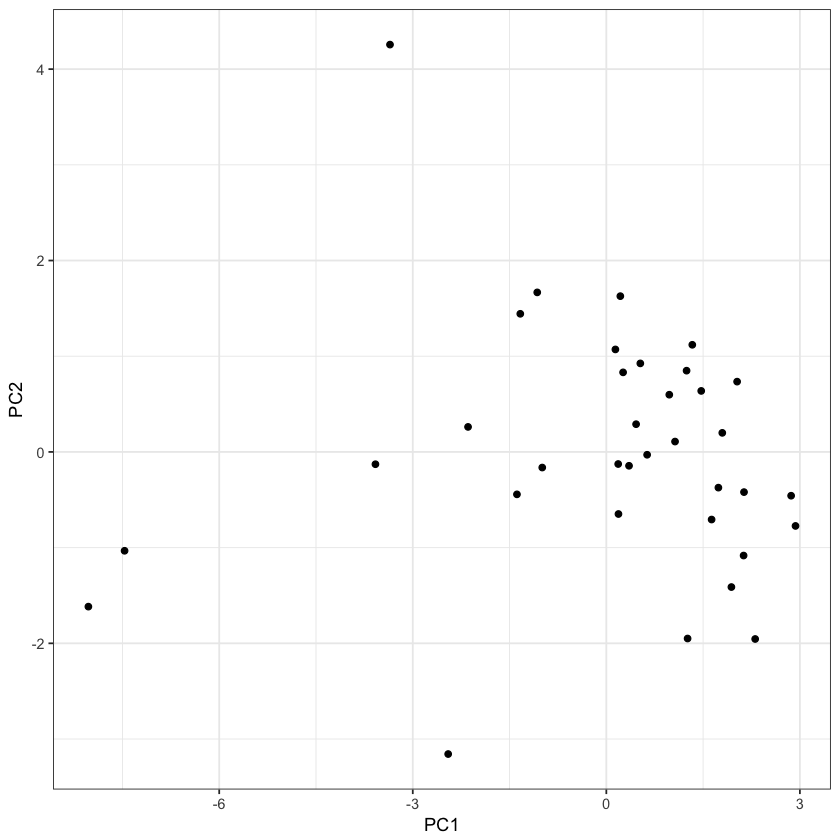
\includegraphics[width=8cm,height=7.5cm]{img/pc.png}
      \caption{各主成分分量的特征值碎石图}
\end{figure}

\subsection{聚类分析}
聚类是将相似的事物聚集在一起,而将不相似的事物划分到不同类别的过程,是数据分析中十分重要的手段。本文采用离差平方和(Ward)法对全国各大重要城市进行系统聚类分析。Ward 法的基本思想是先将 n 个样本各自看成一类,此时离差平方和 W=0,之后每次选取合并之后使得 w 增加最小的两类进行合并,直到所有的样本被合为 1 类, 在 Ward 法中,两类样本合并之后增加的离差平方和为类间距离
$$D_{pq}^2 = W_{r} - (W_p + W_q)$$
其中$D_{pq}^2$ 为聚类分析的类间距离;$W_r$,$W_p$,$W_q$
分别为 r(p类和q类合并成的类),p,q 类样品的离差平方和。


根据主成分分析提取得到的两个主成分解释变量,使用系统聚类的方法对36个城市进行聚类分析可以得到如图3 所示的聚类结构图,为了比较好地对城市进行划分,本文选择将36个城市聚为五类,从图3中的红框标注和表4中可以看到具体的划分情况。

图4则显示了不同的聚类类别在两个主成分解释变量上的分布情况。可以看到类别1和类别5的界限较为明显,比较离群的深圳市被归为第二类,类别2、3、4的界限相对来说比较模糊。

\begin{figure}[h!]
  \centering
         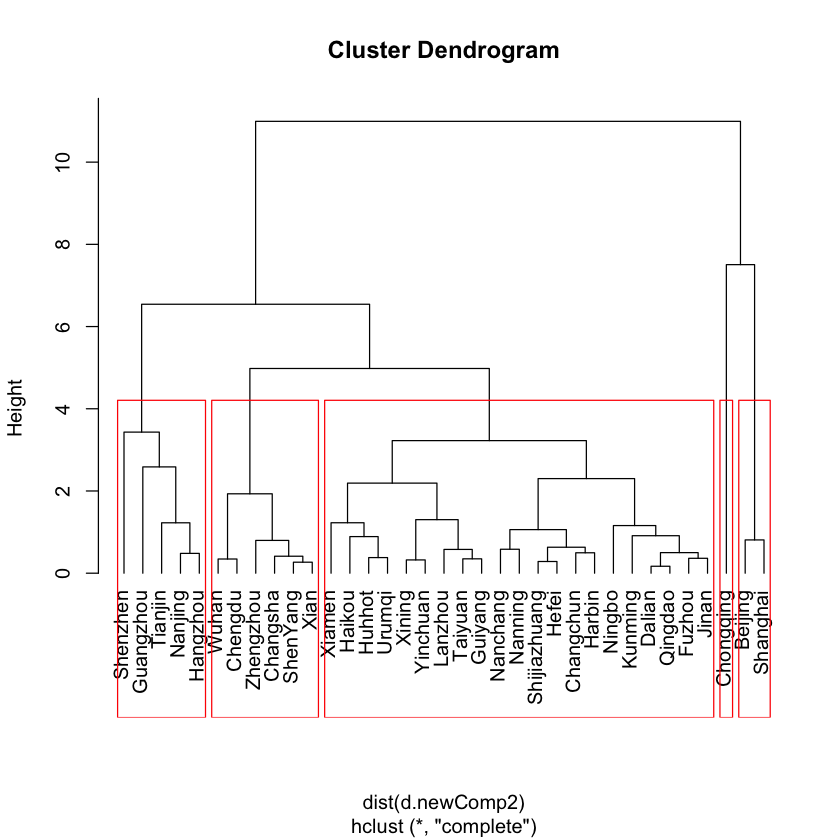
\includegraphics[width=11cm]{img/cluster.png}
      \caption{各聚类类别在主成分分量上的分布}
\end{figure}

\begin{table}[h]
\caption{对全国主要城市进行系统聚类的结果}
\small %此处写字体大小控制
\centering
\begin{tabular}{p{2cm}p{10cm}}
\toprule
类别 & 城市 \\
\midrule
第一类 & 北京、上海 \\ \midrule
第二类 & 天津、南京、杭州、广州、深圳\\ \midrule
第三类 & 石家庄、太原、呼和浩特、 大连、 长春、 哈尔滨、 宁波、 合肥、 福州、 厦门、 南昌、 青岛、 南宁、 海口 、贵阳、 昆明 、兰州、 西宁 、银川 、乌鲁木齐\\ \midrule
第四类 & 沈阳、济南 、郑州、 武汉、 长沙、 成都、 西安\\ \midrule
第五类 & 重庆\\
\bottomrule



\end{tabu}
\end{table}


\begin{figure}[h!]
  \centering
         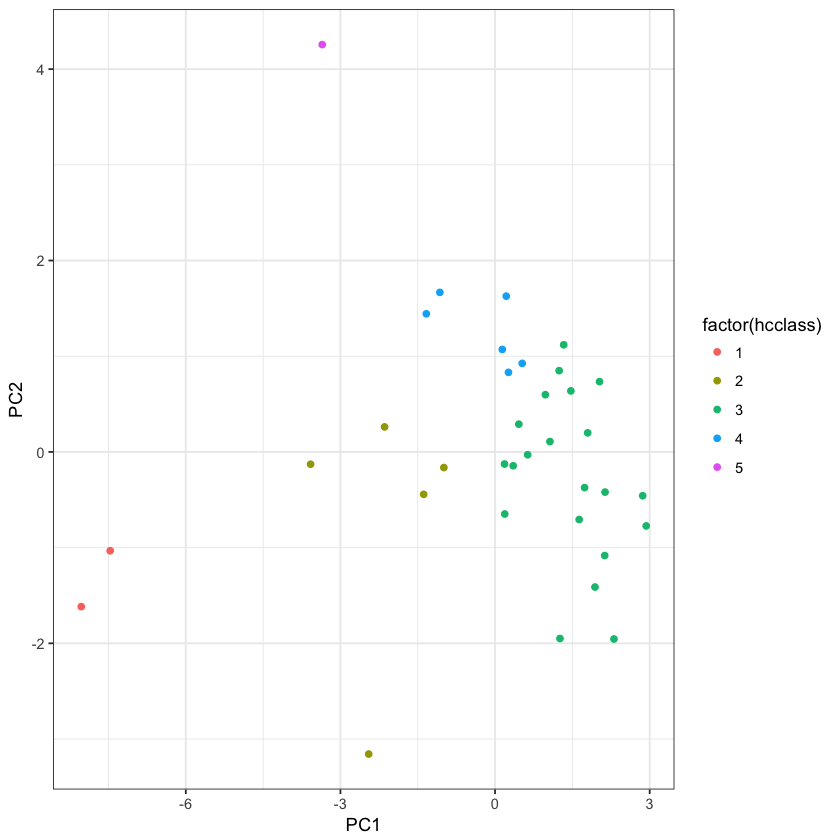
\includegraphics[width=10cm,height=7.5cm]{img/hccluster.png}
      \caption{各聚类类别在主成分分量上的分布}
\end{figure}

\begin{table}[h]
  \centering
  \caption{各聚类类别在各个特征上的均值(标准化之后)}
  \small %此处写字体大小控制
  \begin{tabular}{cccccc}
  \toprule
  &1&2&3&4&5\\
  \midrule
年末总人口	 & 1.15543993 & 	-0.04779539	 & -0.38755766	 & 0.22749761	 & 4.70182229\\
区域生产总值 & 	2.66685447 & 	1.04547808 & 	-0.58608800	 & 0.08824954	 & 1.21725147\\
第三产业占比 & 	1.9889035	 & 0.4282710	 & -0.1274218 & 	-0.4670344 & 	-0.6410972\\
社会商品零售总额 & 	2.8312756 & 	0.8494962	 & -0.5887487 & 	0.2160565 & 	1.1573516\\
地方财政预算内收入	 & 3.37196596 & 	0.61905345 & 	-0.49450184	 & -0.07716431 & 	1.00832527\\
在岗职工平均工资 & 	3.1996157	 & 0.9295291 & 	-0.3946497 & 	-0.3845422 & 	-0.4519794\\
房地产开发投资金额	 & 2.3396028 & 	0.3055734 & 	-0.5932372	 & 0.6209956	 & 2.5249346\\
商品房销售价格 & 	1.9654901	 & 1.3303667 & 	-0.3361090 & 	-0.4599305 & 	-0.7649408\\
普通高等学校在校学生 & 	0.4170865 & 	0.5105537	 & -0.4924249	 & 0.9972016	 & 0.9707719\\
城乡居民储蓄年末余额 & 	3.34949266	 & 0.58462285	 & -0.51595760 & 	0.03082474 & 	1.02806162\\
  \bottomrule
  \end{tabular}
\end{table}



\subsection{结果分析}

根据对全国主要城市进行系统聚类的结果可以发现,被分到第一类的北京、上海作为我国发展最发达的两个特大型城市,相比于其他城市而言人口较多,经济发展水平高,工资高、房价高;被分到第二类的天津、南京、杭州、广州、深圳是我国经济发展水平很高的大城市,相对而言人口较少,经济发达,工资较高,房价较高;被分到第四类的沈阳、济南、郑州、武汉、长沙、成都、西安是我国经济发展非常有活力的省会城市,经济发展较好,房价较低,高校较多;被分到第五类的重庆市经济发展较好,由于人口最多,房价很低跟其他经济发展相当的城市显著区分开来;其他城市被分到第三类,相对而言人口、房价、教育资源和经济发展水平都不及其他类的城市。

\section{判别分析}
判别分析是在分类确定的条件下,根据某一研究对象的各种特征值判别其归属类型的一种统计分析方法。在这一部分中,我们利用Fisher判别分析的方法对全国主要城市的聚类结果进行分析和评估。
\subsection{Fisher判别分析简介}
Fisher判别分析是判别分析的一种方法,其基本思路是通过将空间中的点进行投影变换,根据变换后与其他样本点的亲疏关系判断其类别归属的方法。其本质也是一种降维方法。Fisher判别分析可以分为一下几个步骤:

1) 计算各类样本的均值向量$\mu_i$ 和总样本均值$\bar{\mu}$,$N_i$ 是类$\omega_i$ 的样本个数,$m$为总类别数
$$ \mu_i = \frac{1}{N_i}\sum_{X \omega_i}X ~~ i=1,2,...m$$
$$ \bar{\mu} = \frac{1}{\sum_i^m{N_i}} \sum X$$

2) 计算样本类内散度矩阵$S_i$和总类内散度矩阵$S_w$
$$ S_i = \sum_{X \omega_i} (X-\mu_i)(X-\mu_i)^T ~~ i = 1,2,...n$$
$$ S_w = \sum_{i=1}^m S_i$$

3) 计算样本间离散度矩阵 $S_b$,$S_b = \sum(\mu_i-\bar{\mu})(\mu_i - \bar{\mu})^T$

4) 求向量$a$,为此定义Fisher准则函数
  $$\mathcal{J} (a)= \frac{a'S_ba}{a'S_wa}$$
  使得$\mathcal{J}(a)$取最大值的向量 $a$ 为使$S_w^{-1}S_b$的最大特征值对应的特征向量

5) 对给定样本$x$进行投影, $y = a^Tx$,计算$m$个差值$|y - a^T\mu_i|$,如果存在$k$使得
  $$|y - a^T\mu_k| = \min_{1\le i \le m} |y - a^T \mu_i|$$
  成立,判定$x$属于第$k$类

在Fisher判别分析中,如果一个判别函数不能很好地区分总体,还可以选用多个判别函数,可以选取$S_w^{-1}S_b$的第2大特征值$\lambda_2$ 对应的特征向量$a_2$作为第二判别函数 $y_2 = a_2^Tx$,以此类推可以建立第i大判别函数,每个判别函数的贡献率为$\frac{\lambda_i}{\lambda_1 + \lambda_2 + ... + \lambda_p}$,$p$为特征总数。

\subsection{对聚类结果进行判别分析}
在R语言中使用Fisher判别分析的判别向量载荷如表6所示,各LDA分量的贡献率如表7所示。可以发现第一个LDA分量贡献了75\%的判别,第二项LDA分量贡献了18\%的判别,这两个判别分量是主要判别分量。
所有类别的样本在四个LDA分量上的投影如图5所示,可以发现前两个LDA分量对第一类和第五类样本能进行较好的判别,第三个和第四个LDA分量对于第二、三、四类样本的判别性能较好。
使用留一法对各个城市进行交叉验证之后的结果如表8所示,可以发现总体判别正确率为80\%,判别在第一类和第三类上表现好,在第二类和第四类上表现较差,第五类由于只有一个样本,使用交叉验证的方法并不能正确判别。表9显示了被错误判别的城市的情况。

\begin{table}[h]
  \centering
  \caption{lda分量载荷}
  \small %此处写字体大小控制
  \begin{tabular}{ccccc}
  \toprule
 &LD1 &	LD2	 &LD3	 &LD4\\
  \midrule

年末总人口	 &1.9767775 &		4.7019066 &		-0.1429626 &		1.7826343\\
区域生产总值	 &	8.3313255 &		1.8976473	 &	5.2165209	 &	0.3712513\\
第三产业占比 &		0.4023878 &		0.8651833	 &	0.4168351	 &	0.4501079\\
社会商品零售总额 &		-4.3103947 &		-3.7811492 &	-2.0430650 &		-0.4173809\\
地方财政预算内收入 &		-7.530969	 &	-1.442880	 &	-2.409085	 &	-1.028229\\
在岗职工平均工资 &		-0.2376463 &		1.1917357 &		0.5695342 &		2.0128865\\
房地产开发投资金额 &		0.9284808	 &	0.3514730	 &	0.6058604 &		-1.9908404\\
商品房销售价格 &		0.6492929	 &	0.7344440 &		0.6290248 &		0.5520534\\
普通高等学校在校学生 &		-0.3666272 &		-0.4220067	 &	0.5892178	 &	-0.5368479\\
城乡居民储蓄年末余额 &		-4.1474242 &		-0.5110223 &		-1.9406502 &		-0.5227507\\

  \bottomrule
  \end{tabular}
\end{table}

\begin{table}[h]
  \centering
  \caption{各LDA分量的方差贡献率}
  \small %此处写字体大小控制
  \begin{tabular}{ccccc}
  \toprule
  &LD1&LD2&LD3&LD4\\
  \midrule
  方差贡献率 & 0.7511 & 0.1798 &  0.0386 & 0.0306\\
  \bottomrule
  \end{tabular}
\end{table}
\begin{figure}[h!]
  \centering
         
\includegraphics[width=10cm]{img/lda.png}
      \caption{不同类别在各lda分量上的投影}
\end{figure}

\begin{table}[h]
  \centering
  \caption{使用留一法交叉验证对各个分类的判别结果}
  \small %此处写字体大小控制
  \begin{tabular}{cccccc}
  \toprule
 类别	& 类别总数 & 判别正确数 & 判别错误数 &判别正确率\\
  \midrule
  第一类	& 2 & 2 & 0 &100\% \\
  第二类	& 5 & 2 & 3 &40\% \\
  第三类	& 21 & 20 & 1 &95\% \\
  第四类	& 6 & 4 & 2 &67\% \\
  第五类	& 1 & 0 & 1 &0\% \\
  总计	& 35 & 28 & 7 &80\% \\
  \bottomrule
  \end{tabular}
\end{table}
\begin{table}[h]
  \centering
  \caption{聚类结果和判别不一致的城市}
  \small %此处写字体大小控制
  \begin{tabular}{ccc}
  \toprule
 地区	& 聚类类别	& 	 LDA判别类别\\
  \midrule
  天津	& 	2	& 	4\\
  南京	& 	2	& 	3\\
  杭州		& 2	  & 4\\
  昆明		& 3		& 4\\
  长沙		& 4	& 	3\\
  成都	& 	4	& 	2\\
  重庆 & 5 & NA\\
  \bottomrule
  \end{tabular}
\end{table}


\subsection{结果分析}
通过判别结果可以发现,天津、南京、杭州、昆明、长沙、成都这几个城市的判别结果和聚类结果不一致,猜想可能是由于天津、南京、杭州这三个城市虽然被分到第二类,但是综合来看发展程度不及广深,天津杭州被判别到第四类,南京可能发展程度在这些城市中稍差一些,被判别到第三类。昆明可能在第三类城市中发展程度较好,被归为第四类。成都由第四类被判别为第二类,可能说明其在我国的一二线大城市中有着很强的发展活力。
\end{document}
